\documentclass[osajnl,twocolumn,showpacs,superscriptaddress,10pt]{revtex4-1}
%
\usepackage{dcolumn}% Align table columns on decimal point
\usepackage{bm}% bold math

\usepackage[spanish,es-tabla]{babel}
\usepackage[utf8]{inputenc}
\usepackage[T1]{fontenc}
\usepackage{makeidx}
\usepackage{graphicx}
\usepackage{subfig}
\usepackage{gensymb}
\usepackage{physics}
\usepackage{amsmath}
\usepackage{amsfonts}
\usepackage{amssymb}
\usepackage[pdftex]{hyperref}
\usepackage{multirow}
\usepackage{float}
\usepackage{booktabs}
\usepackage{listingsutf8}
\usepackage{hyperref}
\usepackage{listings}
\usepackage[table,xcdraw]{xcolor}

\definecolor{myblue}{RGB}{0,0,255} % Define your keyword color
%\usepackage[table,xcdraw]{xcolor}
\decimalpoint
%\bibliographystyle{IEEEtran}
%\bibliography{IEEEabrv,mybibfile}
%
%

\begin{document}
%Titulo
\title{Fase 2 -  Sistema de Apoyo en la
Movilidad para una Persona no Vidente}
\thanks{Electronica 6}

\author{Kevin Alexander, Medina Monterroso,\IEEEmembership{ 2019-02084}}\email{e-mail: kevin2000medina14@gmail.com}
\author{Mike Antony Stuardo Medina Guzmán,\IEEEmembership{ 2019-03908} }
\author{Julio Rubén Sanic Martínez,\IEEEmembership{ 2012-22286} Grupo E6\_(B-03) }


\affiliation{Catedrático, Ing. Ligia Deyanira Aguilar, Escuela de Mecánica Eléctrica, Laboratorio de Electrónica 6, Primer Semestre 2023, Universidad San Carlos, Edificio T1, Ciudad Universitaria, Zona 12, Guatemala.}%

%\collaboration{MUSO Collaboration}%\noaffiliation
%\noaffiliation

\date{\today}%

\maketitle{}
%Resumen
\begin{abstract}
El proyecto consiste en crear un sistema para ayudar a personas no videntes a detectar objetos cercanos. Se utilizan dos sensores, uno a la altura de la cintura y otro cerca del suelo, para detectar objetos. Cuando se detecta un objeto, se activa una alarma y se envían datos a un dashboard en tiempo real que muestra información sobre la detección. El sistema se basa en una FPGA y se puede programar en Python y/o JavaScript. El objetivo es mejorar la movilidad y seguridad de las personas no videntes, basando este documento en la fase temprana de estudio del mismo
\end{abstract}


\section{Objetivos}

\subsection{Generales}

\begin{itemize}
\item[*] Realizar un sistema mediante las propuestas analizadas en este documento que permita un sistema de apoyo a personas no videntes.
\end{itemize}

\subsection{Específicos}

\begin{itemize}
\item[*] Describir, mediante el texto analizado y los conocimientos recibidos, la forma de trabajo a futuro en el enfoque al proyecto mencionado.

\item[*] Evaluar los sistemas de índice analógico y digital mediante los avances del proyecto.

\item[*] Evidenciar el trabajo en conjunto de los investigadores, realizando la superposición y conjunción de ideas para la realización del proyecto.

\end{itemize}

\section{Propuesta de algoritmos a utilizar}
La propuesta final consiste en utilizar la FPGA como adquisición de datos de los sensores y manejo de actuadores (alarma), también como medio primario de transmisión para el dispositivo ESP8266, el cual envía la información por medio de websockets a un servidor alojado en Heroku que tiene como backend a node.js y ws (librería para menejar websockets tanto como servidor y cliente) para la comunicación de websockets a un front-end alojado en AWS S3 elaborado con React.js.


\begin{figure}[H]
    \begin{center}
        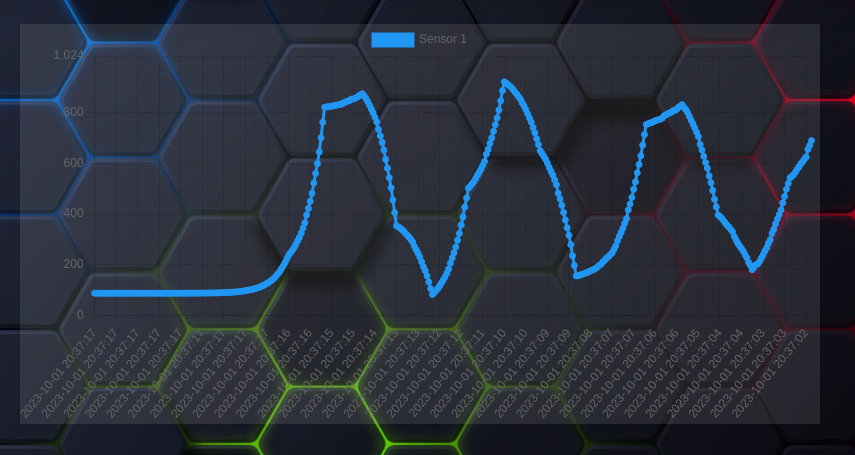
\includegraphics[scale=0.3]{images/Screenshot from 2023-10-01 14-37-32.png}
        \caption{Ejemplo de GUI}
    \end{center}
\end{figure}


\section{Descripción del hardware y software a utilizar.}

\subsection{Lenguaje de programación}

\subsubsection{VHDL}

VHDL, que significa "VHSIC Hardware Description Language" (Lenguaje de Descripción de Hardware de Sistemas Integrados de Muy Alta Velocidad), es un lenguaje de descripción de hardware utilizado para modelar y diseñar circuitos digitales y sistemas electrónicos. VHDL se basa en un conjunto de reglas y sintaxis que permiten a los ingenieros describir el comportamiento y la estructura de un sistema digital de manera precisa y detallada.

\begin{figure}[H]
    \begin{center}
        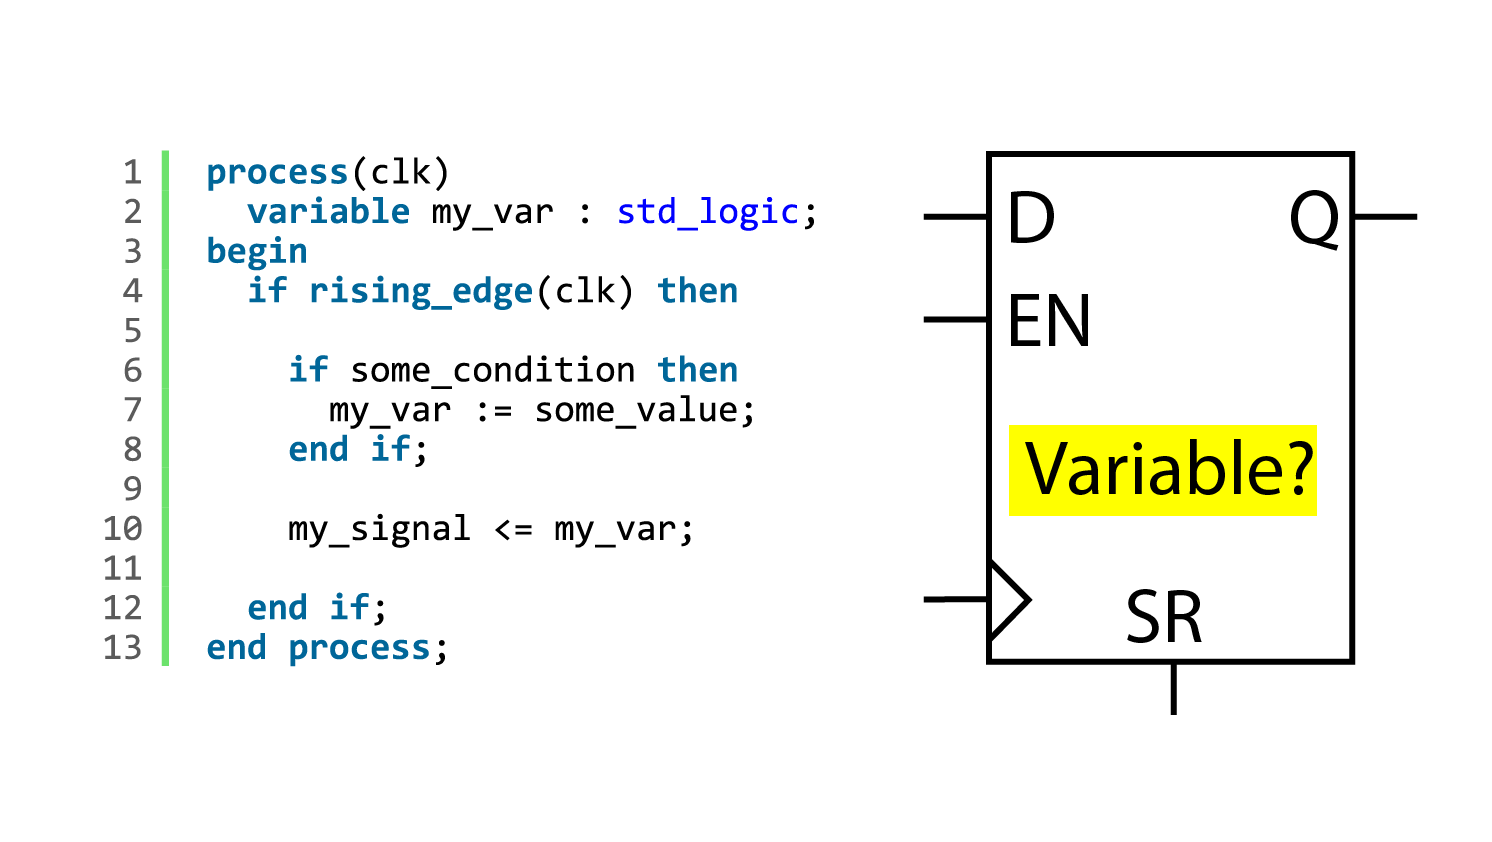
\includegraphics[scale=0.12]{images/variables-as-registers.png}
        \caption{VHDL}
        \label{Amplificador Operacional}
    \end{center}
\end{figure}


En el contexto de ISE 14.7 de Xilinx Corporation, VHDL se utiliza como el lenguaje principal para describir el diseño de hardware digital que se implementará en las FPGA de Xilinx. Los diseñadores utilizan VHDL en ISE para definir la funcionalidad de los módulos y circuitos digitales, así como para especificar cómo estos componentes se conectan entre sí. ISE 14.7 proporciona un entorno de desarrollo que permite a los ingenieros sintetizar, simular y verificar sus diseños VHDL antes de cargarlos en la FPGA para su implementación en hardware físico.


\subsection{JavaScript}

JavaScript es un lenguaje de programación versátil y de alto nivel que se utiliza para el desarrollo web y más. Es conocido por su capacidad para agregar interactividad a sitios web, ejecutarse en navegadores web y usarse para programación del lado del servidor. JavaScript se escribe dinámicamente, admite paradigmas de programación funcional, imperativo y orientado a objetos, y tiene un rico ecosistema de bibliotecas y marcos. Es esencial para el desarrollo web moderno y es compatible con los principales navegadores web.
\\

\section*{Librerías y Herramientas para el Proyecto}

\subsection*{Programación de FPGA con ISE 14.7}

\begin{itemize}
    \item \textbf{VHDL/Verilog}: VHDL y Verilog son los lenguajes de descripción de hardware estándar para la programación de FPGAs en ISE 14.7. Se utilizan para diseñar y describir el comportamiento de los módulos de hardware.
\end{itemize}

\subsection*{Adquisición de Datos en FPGA}

\begin{itemize}
  \item \textbf{Librerías de Xilinx para FPGA}: ISE 14.7 proporciona una serie de librerías y componentes predefinidos que pueden ser útiles para la adquisición de datos, como las relacionadas con la interfaz de comunicación con sensores y la conversión analógico-digital (ADC).
\end{itemize}

\subsection*{Procesamiento de Datos en FPGA}

\begin{itemize}
  \item \textbf{Librerías VHDL/Verilog personalizadas}: Se deben desarrollar librerías personalizadas en VHDL/Verilog para implementar algoritmos específicos de procesamiento de datos en la FPGA. Estas librerías personalizadas pueden incluir operaciones matemáticas, filtros, detección de objetos, etc.
\end{itemize}

\subsection*{Interfaz de Usuario en ReactJS (JavaScript Frontend)}

\begin{itemize}
  \item \textbf{chart.js}: 
  Chart.js es una biblioteca de JavaScript para crear cuadros y gráficos interactivos y visualmente atractivos en páginas web. Proporciona una API fácil de usar para crear varios tipos de gráficos, incluidos gráficos de barras, gráficos de líneas, gráficos circulares y más. Con Chart.js, se puede personalizar la apariencia del gráfico, manejar las interacciones del usuario y mostrar datos de una manera visualmente atractiva. Se usa ampliamente para la visualización de datos y es compatible con tecnologías web modernas como HTML5 y Canvas.
  \item \textbf{react-chartjs-2}:
  react-chartjs-2 es un contenedor de React para la biblioteca Chart.js. Le permite integrar fácilmente cuadros y gráficos de Chart.js en aplicaciones React. Con react-chartjs-2, se puede crear gráficos interactivos y personalizables mientras aprovecha el poder de la arquitectura basada en componentes de React. Simplifica el proceso de creación y actualización de gráficos en aplicaciones React, lo que hace que la visualización de datos sea sencilla y eficiente.
  \item \textbf{react-redux}:
  react-redux es una biblioteca para integrar Redux, una biblioteca de gestión de estado, en aplicaciones React. Proporciona una forma de conectar sus componentes de React a una tienda Redux, lo que le permite acceder y actualizar el estado de la aplicación utilizando principios de Redux como acciones y reductores.

  \item \textbf{@reduxjs/toolkit}:
  @reduxjs/toolkit es una biblioteca oficial para Redux que simplifica las tareas comunes de Redux. Proporciona utilidades para definir reductores, acciones y configuración de la tienda de una manera más concisa y eficiente, reduciendo el código repetitivo. Fomenta las mejores prácticas y ayuda a los desarrolladores a escribir código Redux más limpio y más fácil de mantener.
  
  \item \textbf{framer-motion}:
  Framer Motion es una biblioteca de animación popular para aplicaciones React. Simplifica el proceso de agregar animaciones a elementos web, facilitando la creación de interfaces de usuario fluidas e interactivas. Con Framer Motion, se puede animar componentes, transiciones y gestos, mejorando la experiencia general del usuario en aplicaciones React. Es conocido por su sintaxis declarativa y su flexibilidad, lo que hace que las animaciones complejas sean más accesibles para los desarrolladores.
\end{itemize}

\subsection*{Servidor para comunicación de Websockets (JavaScript backend)}
\begin{itemize}
    \item \textbf{node.js}: 
    Node.js es un entorno de ejecución de JavaScript que permite a los desarrolladores ejecutar código JavaScript fuera de los navegadores web. Es conocido por sus capacidades del lado del servidor, que permiten la creación de aplicaciones de red escalables y eficientes. Node.js está controlado por eventos y no bloquea, lo que lo hace adecuado para crear aplicaciones y API en tiempo real. Tiene un vasto ecosistema de paquetes y bibliotecas disponibles a través de npm, lo que simplifica las tareas de desarrollo. Node.js se usa ampliamente para servidores web, herramientas de línea de comandos y aplicaciones de IoT.
    \item \textbf{ws}:
    El paquete ws en Node.js es una biblioteca que proporciona soporte WebSocket para crear comunicación bidireccional en tiempo real entre un servidor y los clientes. Le permite crear servidores y clientes WebSocket, lo que facilita la implementación de funciones como chat en vivo, notificaciones o cualquier aplicación que requiera intercambio de datos de baja latencia.
    \\
    Las características clave del paquete ws incluyen soporte para el protocolo WebSocket, manejo eficiente de conexiones y una API sencilla para crear servidores y clientes WebSocket en Node.js. Se utiliza comúnmente para mejorar la interactividad y las capacidades en tiempo real de aplicaciones y servicios web.

\end{itemize}



\subsection*{Comunicación entre FPGA y esp8266}

\begin{itemize}
  \item \textbf{Librerías de comunicación personalizadas}: Debe implementarse protocolos de comunicación personalizados en la FPGA y JavaScript para permitir la transferencia de datos en tiempo real entre ambos.
\end{itemize}



En resumen, este proyecto involucra una combinación de librerías y herramientas en diferentes entornos: ISE 14.7 para la programación de la FPGA, 
JavaScript tanto para el backend y frontend de la comunicación de websockets.

\subsection{Materiales propuestos}


\textbf{FPGA (Field-Programmable Gate Array) }es un dispositivo de hardware reconfigurable que permite a los diseñadores crear circuitos digitales personalizados mediante programación. A diferencia de los microcontroladores, las FPGA pueden adaptarse a una amplia variedad de aplicaciones y algoritmos mediante la programación de su lógica interna. Se utilizan en aplicaciones donde se requiere un alto rendimiento y flexibilidad, como procesamiento de señales, aceleración de algoritmos, diseño de hardware específico y emulación de sistemas. Las FPGA se utilizan en campos como la electrónica de consumo, la industria aeroespacial y la investigación científica.

\begin{figure}[H]
\begin{center}
    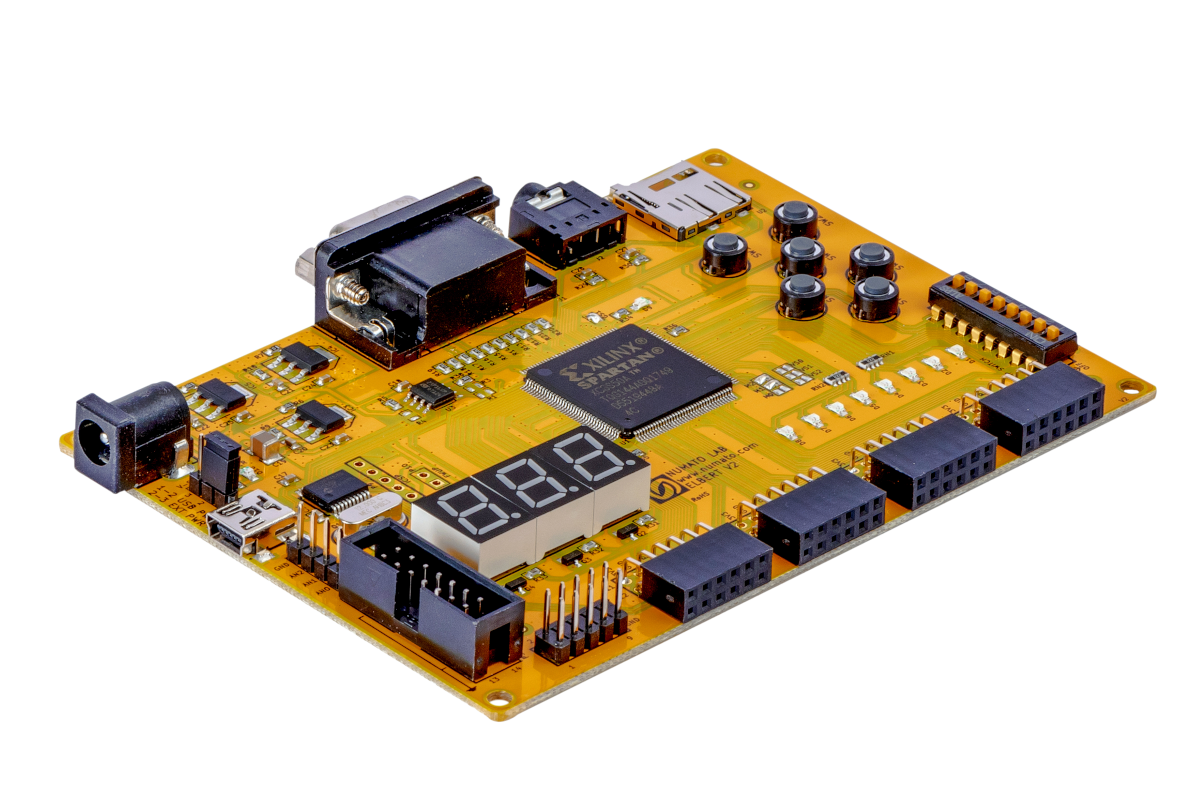
\includegraphics[scale=0.8]{images/ElbertV2_2-2-1-A.png}
    \end{center}
\end{figure}

\textbf{El ESP8266} es un módulo de bajo costo y bajo consumo de energía que integra un microcontrolador y Wi-Fi. Es ampliamente utilizado en proyectos de Internet de las cosas (IoT) debido a su capacidad para conectarse a redes Wi-Fi y su facilidad de programación. El ESP8266 se utiliza para crear dispositivos IoT como sensores, cámaras de seguridad, termostatos inteligentes y sistemas de control remoto. Su flexibilidad y asequibilidad lo convierten en una opción popular en la creación de prototipos y proyectos finales.

\begin{figure}[H]
\begin{center}
    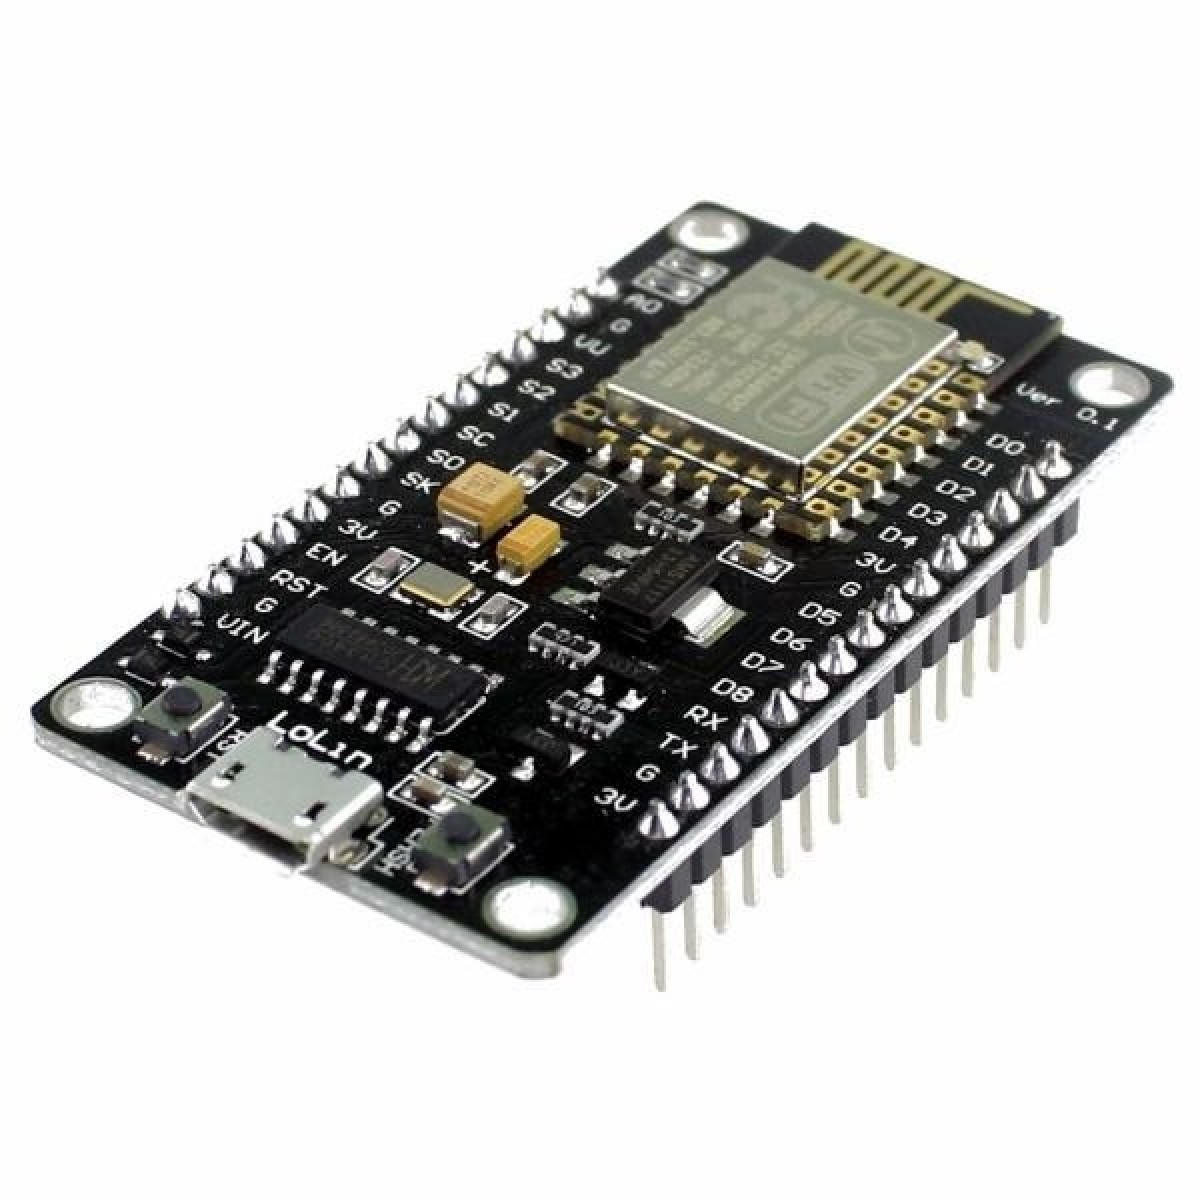
\includegraphics[scale=0.15]{images/MODULO-WI-FI-NODEMCU-ESP8266-1200x1200.jpg}
    \end{center}
\end{figure}

\textbf{El Sensor Ultrasónico} es un dispositivo que utiliza ondas sonoras de alta frecuencia para medir distancias. Emite un pulso de ultrasonido y mide el tiempo que tarda en rebotar en un objeto y regresar al sensor. Esta medición se utiliza para determinar la distancia entre el sensor y el objeto. Los sensores ultrasónicos se utilizan comúnmente en aplicaciones como sistemas de estacionamiento automático de automóviles, medidores de nivel de líquido, sistemas de evitación de obstáculos para robots y dispositivos de medición de distancia sin contacto.

\begin{figure}[H]
\begin{center}
    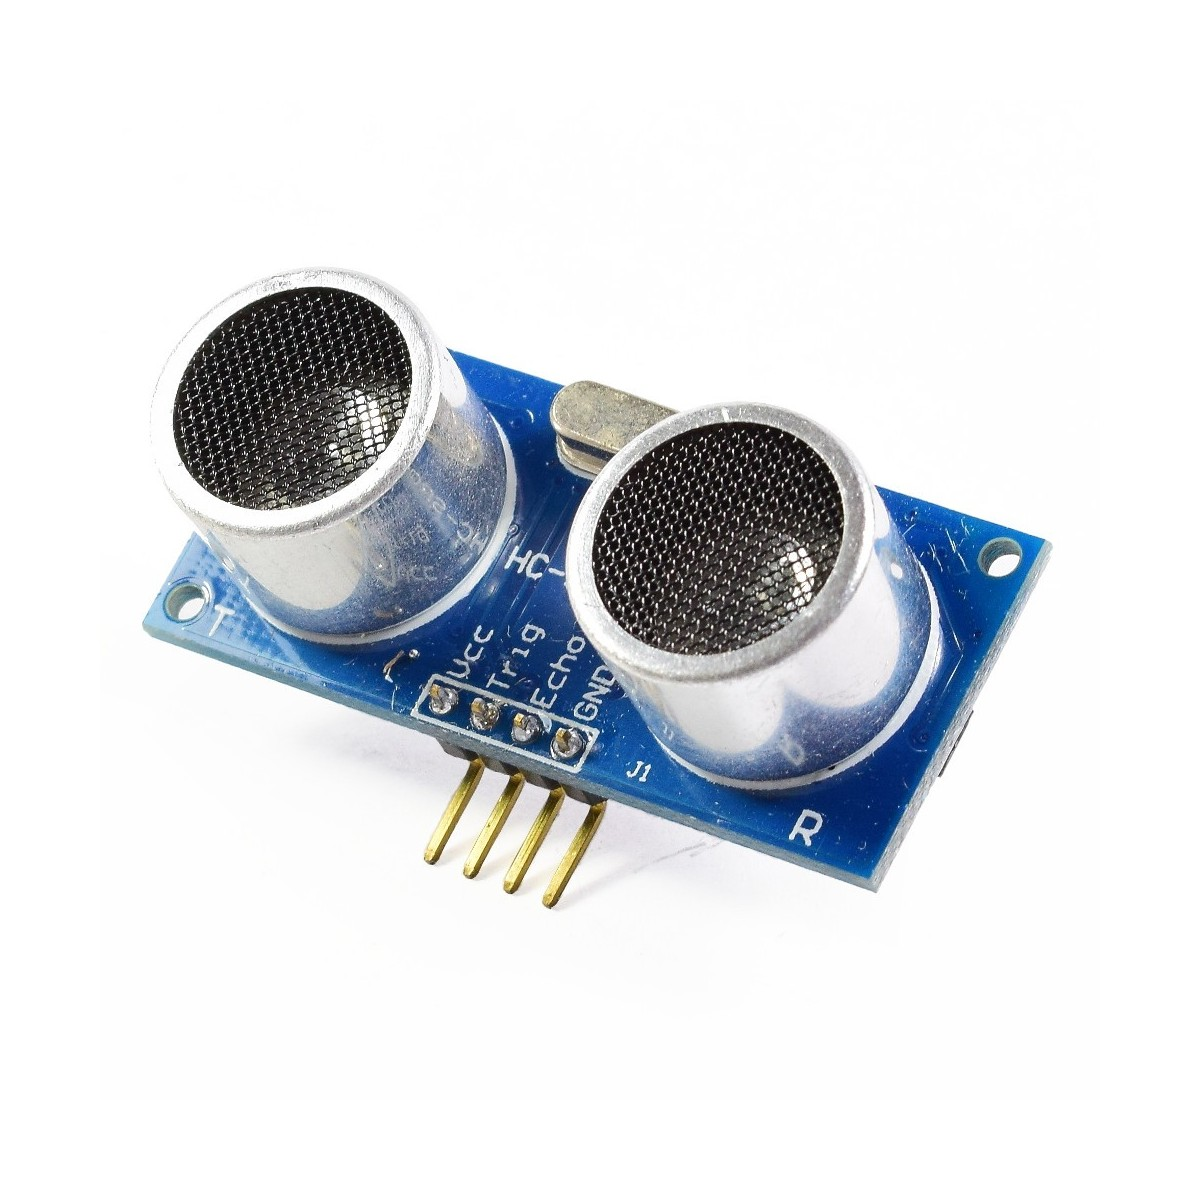
\includegraphics[scale=0.15]{images/sensor-ultrasonido-hc-sr04.jpg}
    \end{center}
\end{figure}


Traslado del circuito a PCB u cambio de estética al montaje del sistema de ayuda visual, análisis del uso de la interfaz gráfica.


\section{Breve descripción de los módulos a implementar en la FPGA}
\begin{itemize}
    \item \textbf{Módulo de Adquisición de Datos:} Este módulo se encargará de leer los datos de los sensores y enviarlos al procesamiento en la FPGA. La FPGA deberá contar con interfaces específicas para adquirir datos de los sensores, como sensores ultrasónicos e infrarrojos. Los datos adquiridos se transmitirán al módulo de procesamiento para su análisis.
    
    \item \textbf{Módulo de Procesamiento de Datos:} Aquí se implementarán algoritmos para procesar los datos de los sensores. Los algoritmos deben calcular la distancia a los objetos detectados, identificar objetos cercanos y determinar sus coordenadas en el espacio. Esto implica realizar cálculos matemáticos y lógicos para interpretar los datos de los sensores y generar información útil para la navegación y detección de obstáculos.
    
    \item \textbf{Módulo de Comunicación:} Este módulo se encargará de establecer la comunicación entre la FPGA y la ESP8266. Puede utilizar interfaces de comunicación como UART (Universal Asynchronous Receiver-Transmitter) o SPI (Serial Peripheral Interface), dependiendo de la elección de hardware. La comunicación bidireccional permitirá enviar datos desde la FPGA al sistema de visualización y recibir comandos o actualizaciones desde el sistema de visualización.
    
    \item \textbf{Módulo de Visualización en Tiempo Real:} Este módulo se utilizará para mostrar los gráficos de radar y la tabla en tiempo real en el dashboard. La visualización en tiempo real es esencial para proporcionar información en tiempo real al usuario no vidente y mejorar su movilidad y seguridad.
\end{itemize}
\section{Diseño Experimental}

El proyecto consiste en un sistema de apoyo para personas no videntes, el diseño del circuito propuesto se analiza tal como se postula en la propuesta de proyecto, mediante dos partes válidas, la primera siendo una interfaz de identificación del sensor, donde se indicara por medio de sus coordenadas la distancia del objeto que se detectó. Mientras, la segunda interfaz se basara plenamente en la muestra de gráficos de radar de los sensores, donde mediante el análisis de los datos de los sensores se presentaran así ambas graficas.\\

El análisis del sistema de diseño se basa en la idea de este comportamiento diagramado por medio del flujo de las ideas centrales de ambas interfaces y el concepto de tiempo para la realización del mismo:\\

\subsection{Presupuesto y materiales a utilizar.}

A partir del análisis de las propuestas y el estudio para la resolución del proyecto se estima que el presupuesto a necesitar, sin contar los gastos ya realizados y piezas comunes, como objetos necesitados en la estructura formada:

\begin{table}[H]
\begin{center}
\begin{tabular}{|cc|c|}
\hline
\rowcolor[HTML]{FE0000} 
\multicolumn{1}{|c|}{\cellcolor[HTML]{FE0000}{\color[HTML]{FFFFFF} \textbf{\begin{tabular}[c]{@{}c@{}}Cantidad \\ Unitaria\end{tabular}}}} &
  {\color[HTML]{FFFFFF} \textbf{Nombre del Producto}} &
  {\color[HTML]{FFFFFF} \textbf{Precio (Q)}} \\ \hline
\multicolumn{1}{|c|}{\textit{\textbf{1}}}  & \begin{tabular}[c]{@{}c@{}}MD-FPGAX006 Elbert V2 \\  Spartan 3A FPGA\end{tabular}   & 510.00  \\ \hline
\multicolumn{1}{|c|}{\textit{\textbf{1}}}  & \begin{tabular}[c]{@{}c@{}}Arduino MEGA 2560 \\ A000067G generic \end{tabular}   & 200.00  \\ \hline
\multicolumn{1}{|c|}{\textit{\textbf{1}}}  & \begin{tabular}[c]{@{}c@{}}Juego jumpers = dupont \\ 80 Cables\end{tabular}    & 55.00   \\ \hline
\multicolumn{1}{|c|}{\textit{\textbf{10}}}  & Led Varias 3mm                                                              & 1.00    \\ \hline
\multicolumn{1}{|c|}{\textit{\textbf{1}}}  & Módulo ESP8266 NodeMcu WIFI                                                 & 95.00    \\ \hline
\multicolumn{1}{|c|}{\textit{\textbf{2}}}  & \begin{tabular}[c]{@{}c@{}}Micro Switch Push \\ Botton 2 Pines\end{tabular}    & 2.50    \\ \hline
\multicolumn{1}{|c|}{\textit{\textbf{2}}} & \begin{tabular}[c]{@{}c@{}}Sensor Infrarrojo \\ IR FC-51 \end{tabular}           & 20.00   \\ \hline
\multicolumn{1}{|c|}{\textit{\textbf{2}}}  & \begin{tabular}[c]{@{}c@{}}Sensor Ultrasonico  \\ ARDUINO HC-SR04 \end{tabular}    & 27.00    \\ \hline
\multicolumn{1}{|c|}{\textit{\textbf{1}}}  & Protoboard de 1 galleta                                                        & 45.00   \\ \hline
\multicolumn{2}{|c|}{\cellcolor[HTML]{96FFFB}\textbf{Cantidad Total}}                                                       & Q1014.00 \\ \hline
\end{tabular}
\end{center}
\end{table}


\subsection{Cronograma}

Basado en el sistema propuesto, se analiza las fechas de entrega de las fases del sistema como la estimación simple de las actividades propuestas.\\

\begin{figure}[H]
    \centering
    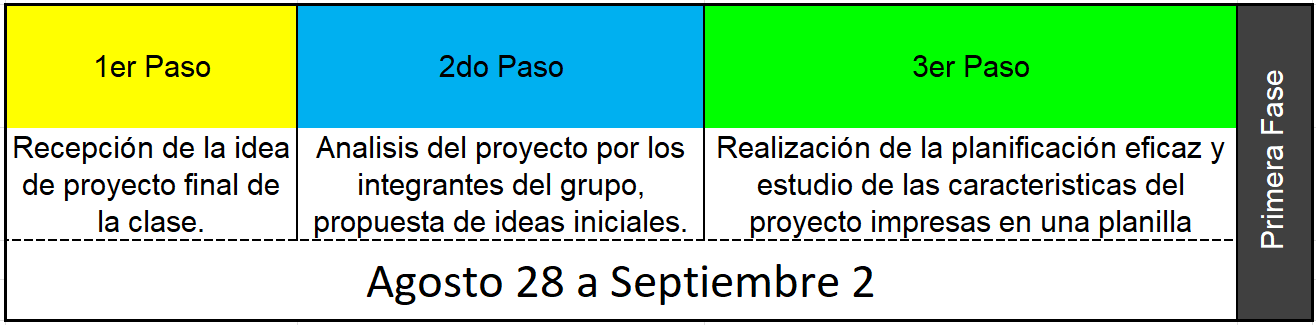
\includegraphics[scale=0.31]{images/CAR1.png}
    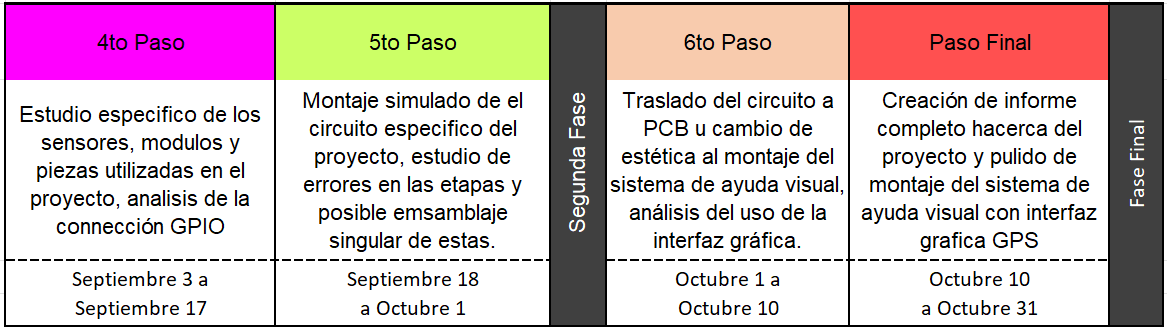
\includegraphics[scale=0.35]{images/CAR2.png}
    \caption{Cronograma de actividades para realización de proyecto.}
    \label{fig:my_label}
\end{figure}

\subsection{Diagrama de Bloques}

Analizando el funcionamiento requerido en el proyecto, se estima la interpretación gráfica por medio de diagrama de bloques basado en las propuestas realizadas en la electrónica futura del circuito. 

\begin{figure}[H]
    \centering
        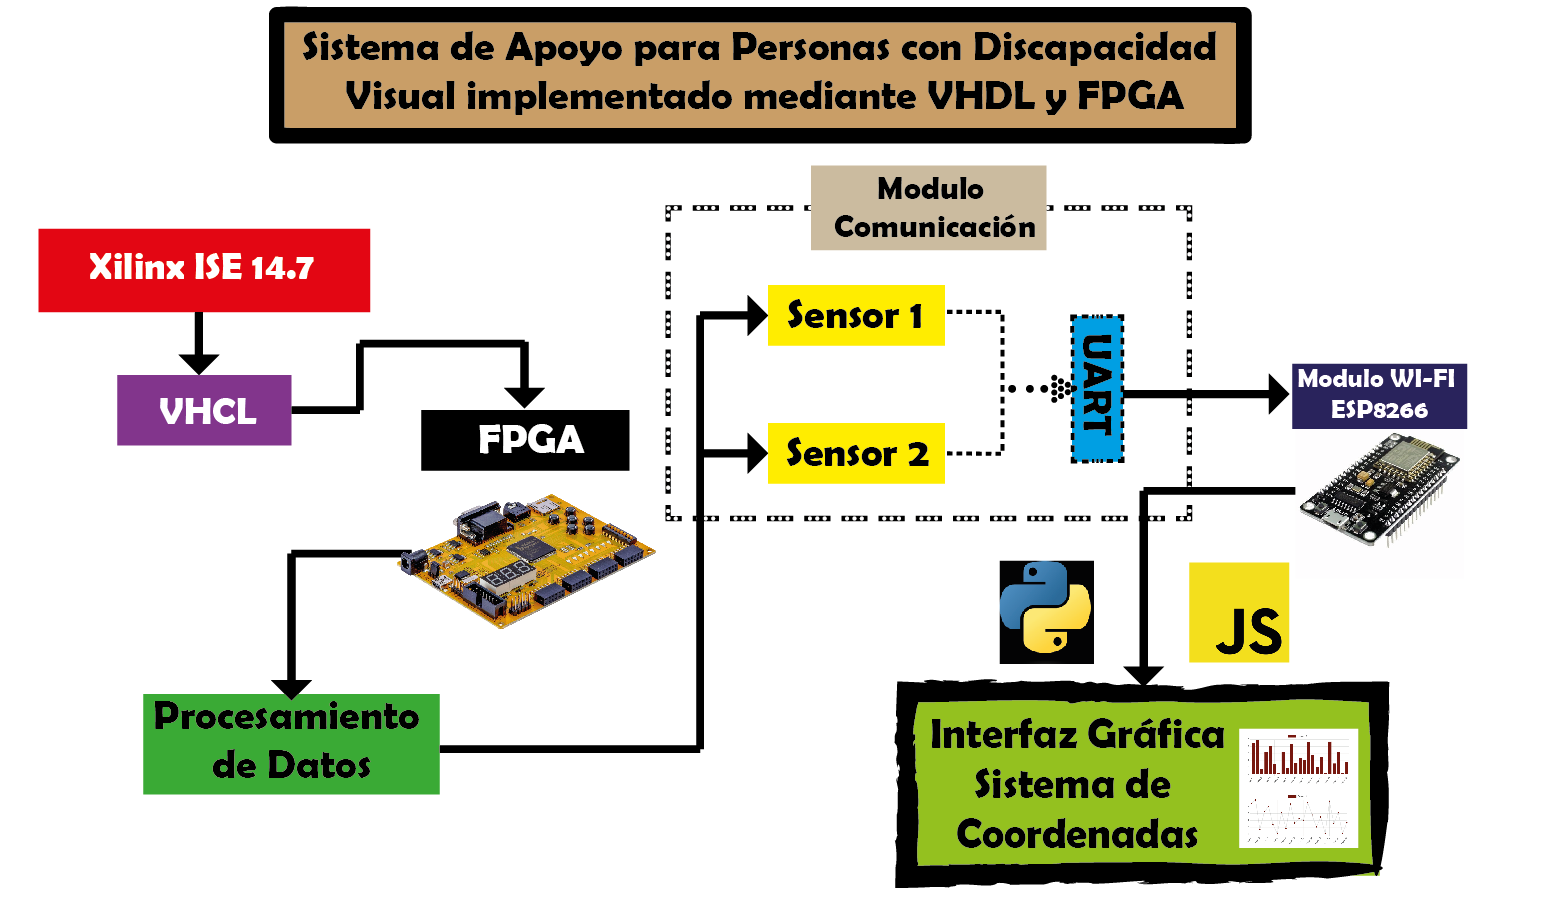
\includegraphics[scale=0.29]{images/Mapa de flujo.png}
    \caption{Diagrama de Bloques del Proyecto}
    \label{fig:my_label}
\end{figure}


\section{Resultados}

\subsection{UART}

El análisis de los datos entre una fpga entrantes por uart es clave para la investigación y conclusión del proyecto, razón a ello se realizan las pruebas básicas de conexión uart, en este caso con un Arduino mega, estableciendo el envío de bits para la realización de un conteo en el display de la elbert V2 

El código de envío de Arduino que responde al contador de nueva usado para la fpga es el siguiente, analizar que se puede enviar cualquier dato, pero se realizó las pruebas mediante este:


\begin{figure}[H]
    \centering
    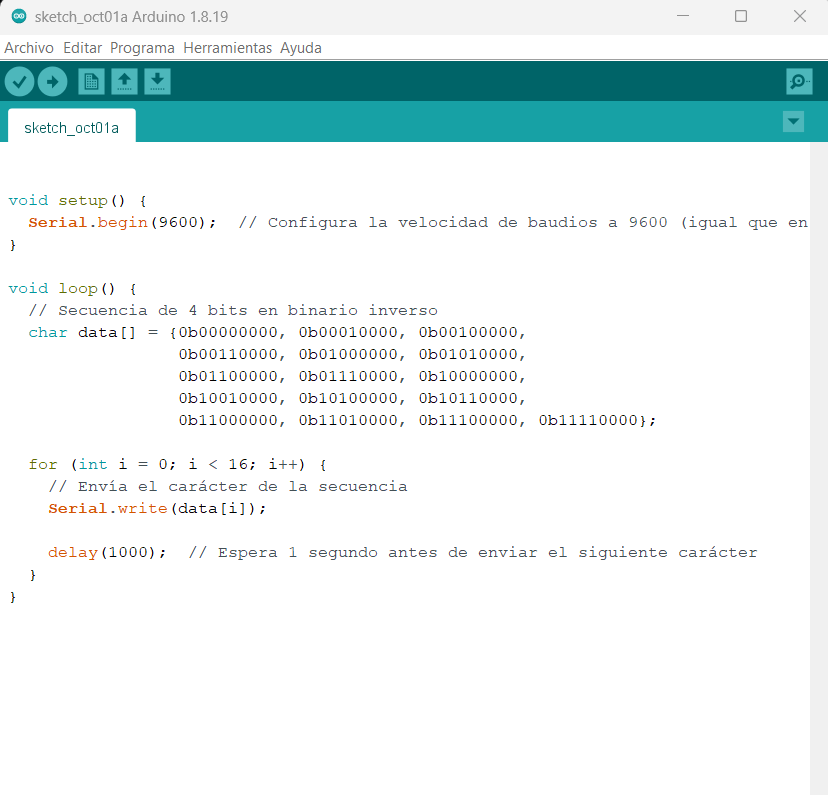
\includegraphics[scale=0.4]{images/codex ardui.png}
    \caption{Código Arduino}
\end{figure}

El análisis de los factores de tx y rx es importante en cuanto al código de la fpga, pues razón a estos mediante el VHDL se puede hacer la conexión directa con la fpga. 

\begin{figure}[H]
    \centering
    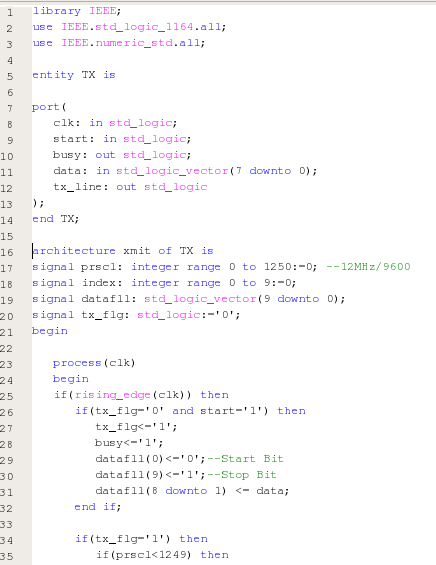
\includegraphics[scale=0.4]{images/tx1.png}
    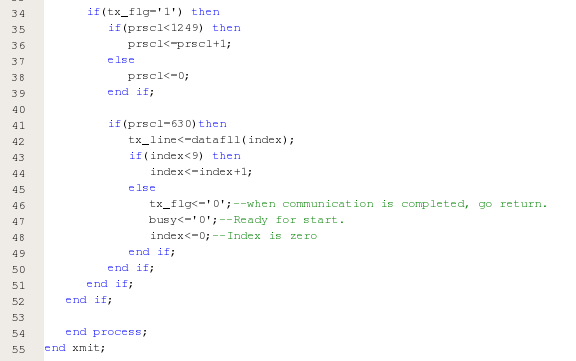
\includegraphics[scale=0.4]{images/tx2.png}
    \caption{Código TX VHDL}
\end{figure}

\begin{figure}[H]
    \centering
    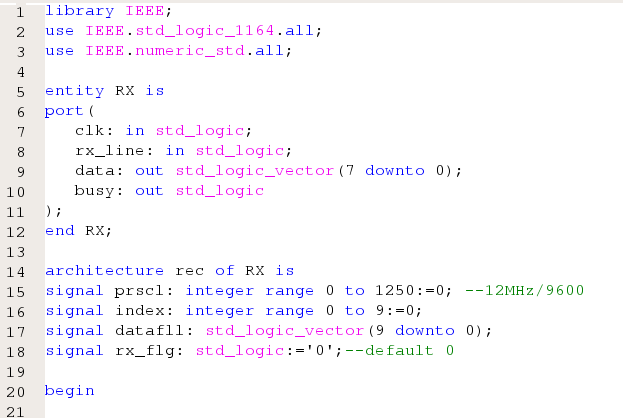
\includegraphics[scale=0.4]{images/rx1.png}
    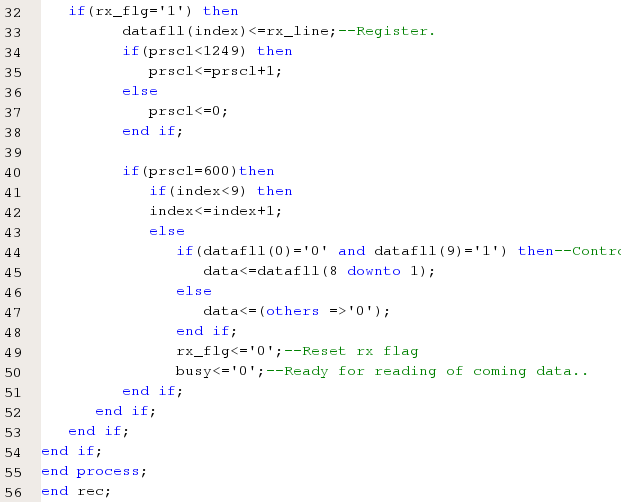
\includegraphics[scale=0.4]{images/rx2.png}
    \caption{Código RX VHDL}
\end{figure}

La pruebas respecto a los leds y el display de 7 segmentos se corresponden al código de multiplexación y él el Arduino conectado, a continuación se presenta la agrupación de estos códigos y la muestra final.

\begin{figure}[H]
    \centering
    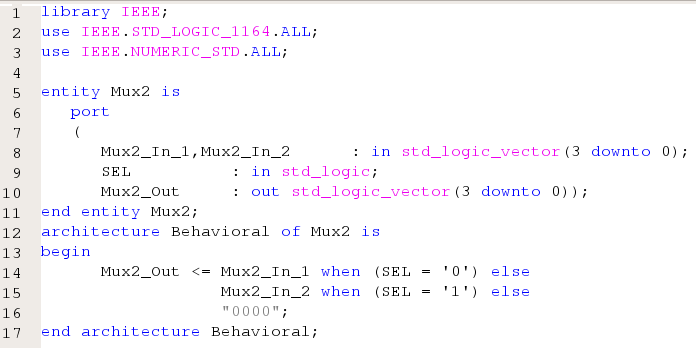
\includegraphics[scale=0.4]{images/mutiplexer.png}
    \caption{Multiplexación}
\end{figure}

\begin{figure}[H]
    \centering
    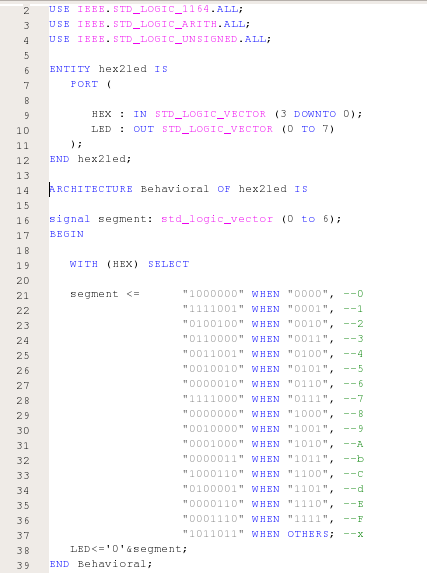
\includegraphics[scale=0.4]{images/7segment.png}
    \caption{7 segmentos}
\end{figure}


\begin{figure}[H]
    \centering
    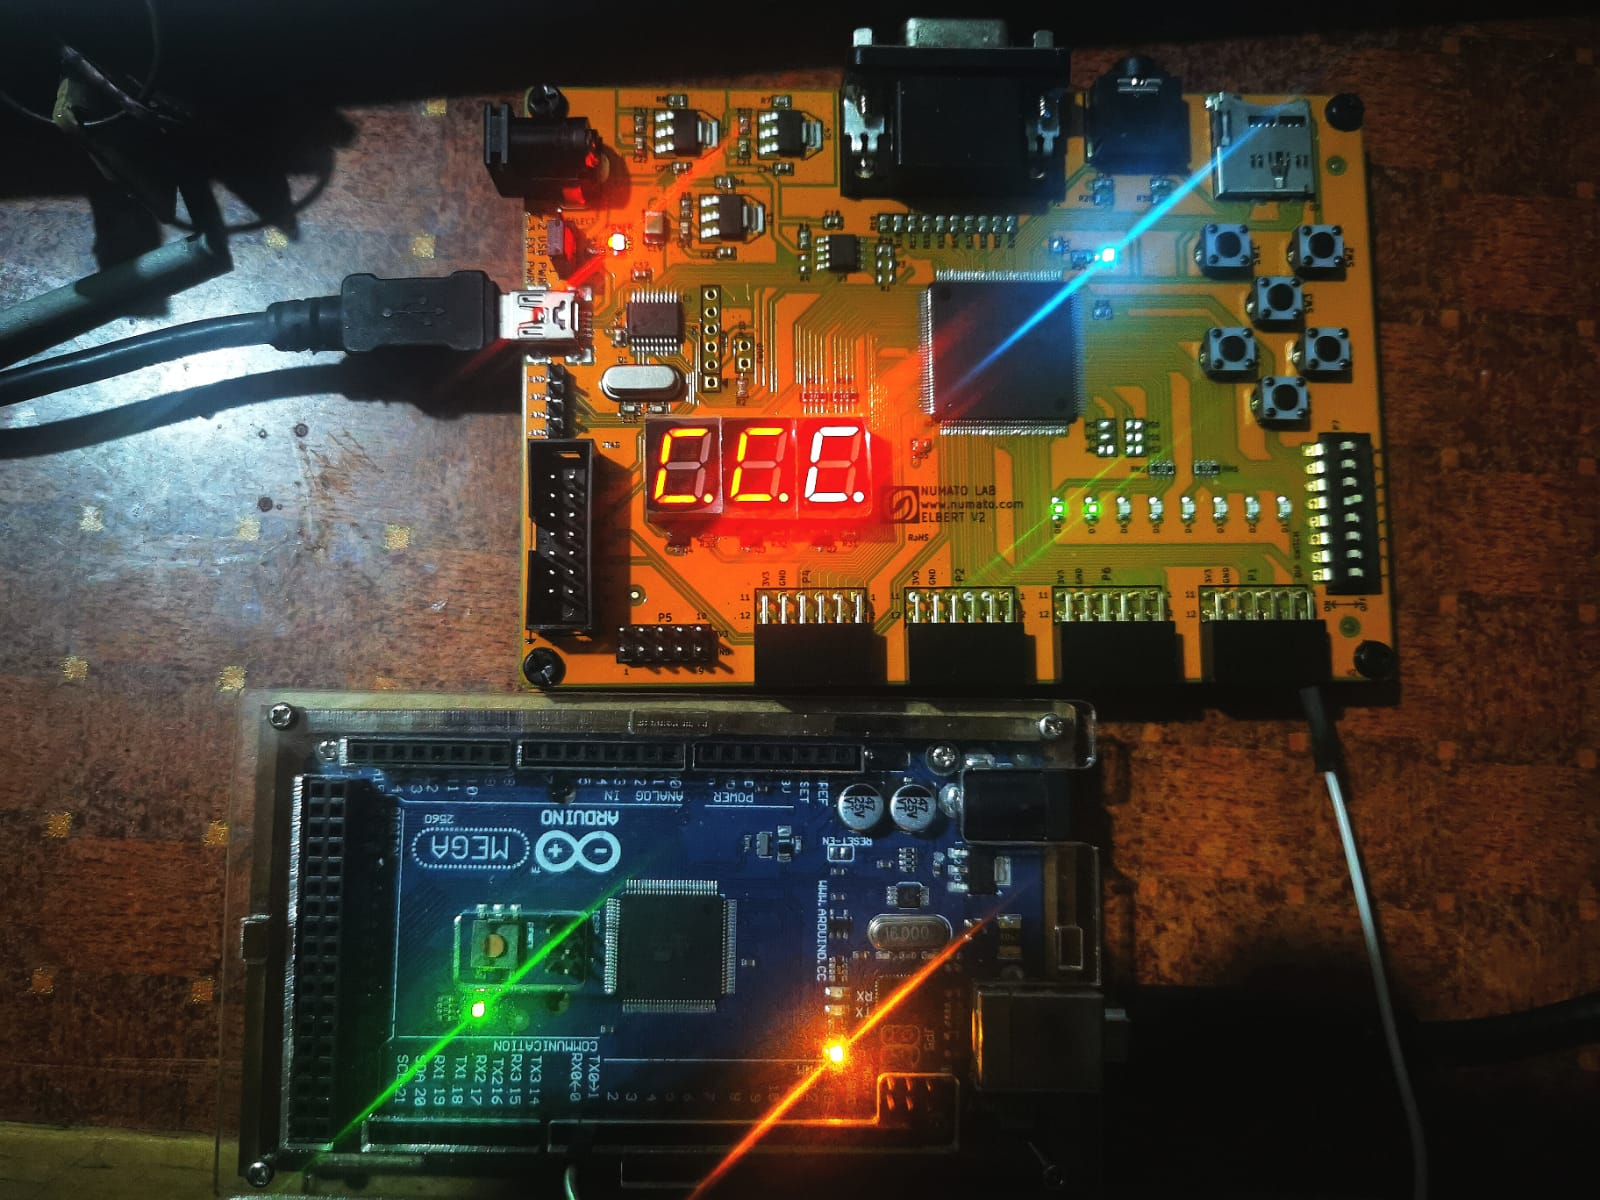
\includegraphics[scale=0.1]{images/WhatsApp Image 2023-10-01 at 3.32.39 AM.jpeg}
    \caption{Resultado UART 7 segmentos}
\end{figure}

\subsection{Transmisión de datos inalámbrico con ESP8266}
Por el momento se tiene una interfaz gráfica en aws - s3 en \url{http://laboratorio-e6.juliosanic.me} para la visualización de datos y un backend en heroku \url{https://apli2-websocket-7abce11f887c.herokuapp.com/} donde se envía la información desde el esp8266 al servidor y de este para la interfaz gráfica.
\\\\
Como se menciona en la sección \ref{sec:Propuesta de algoritmos a utilizar}


\begin{figure}[H]
    \centering
    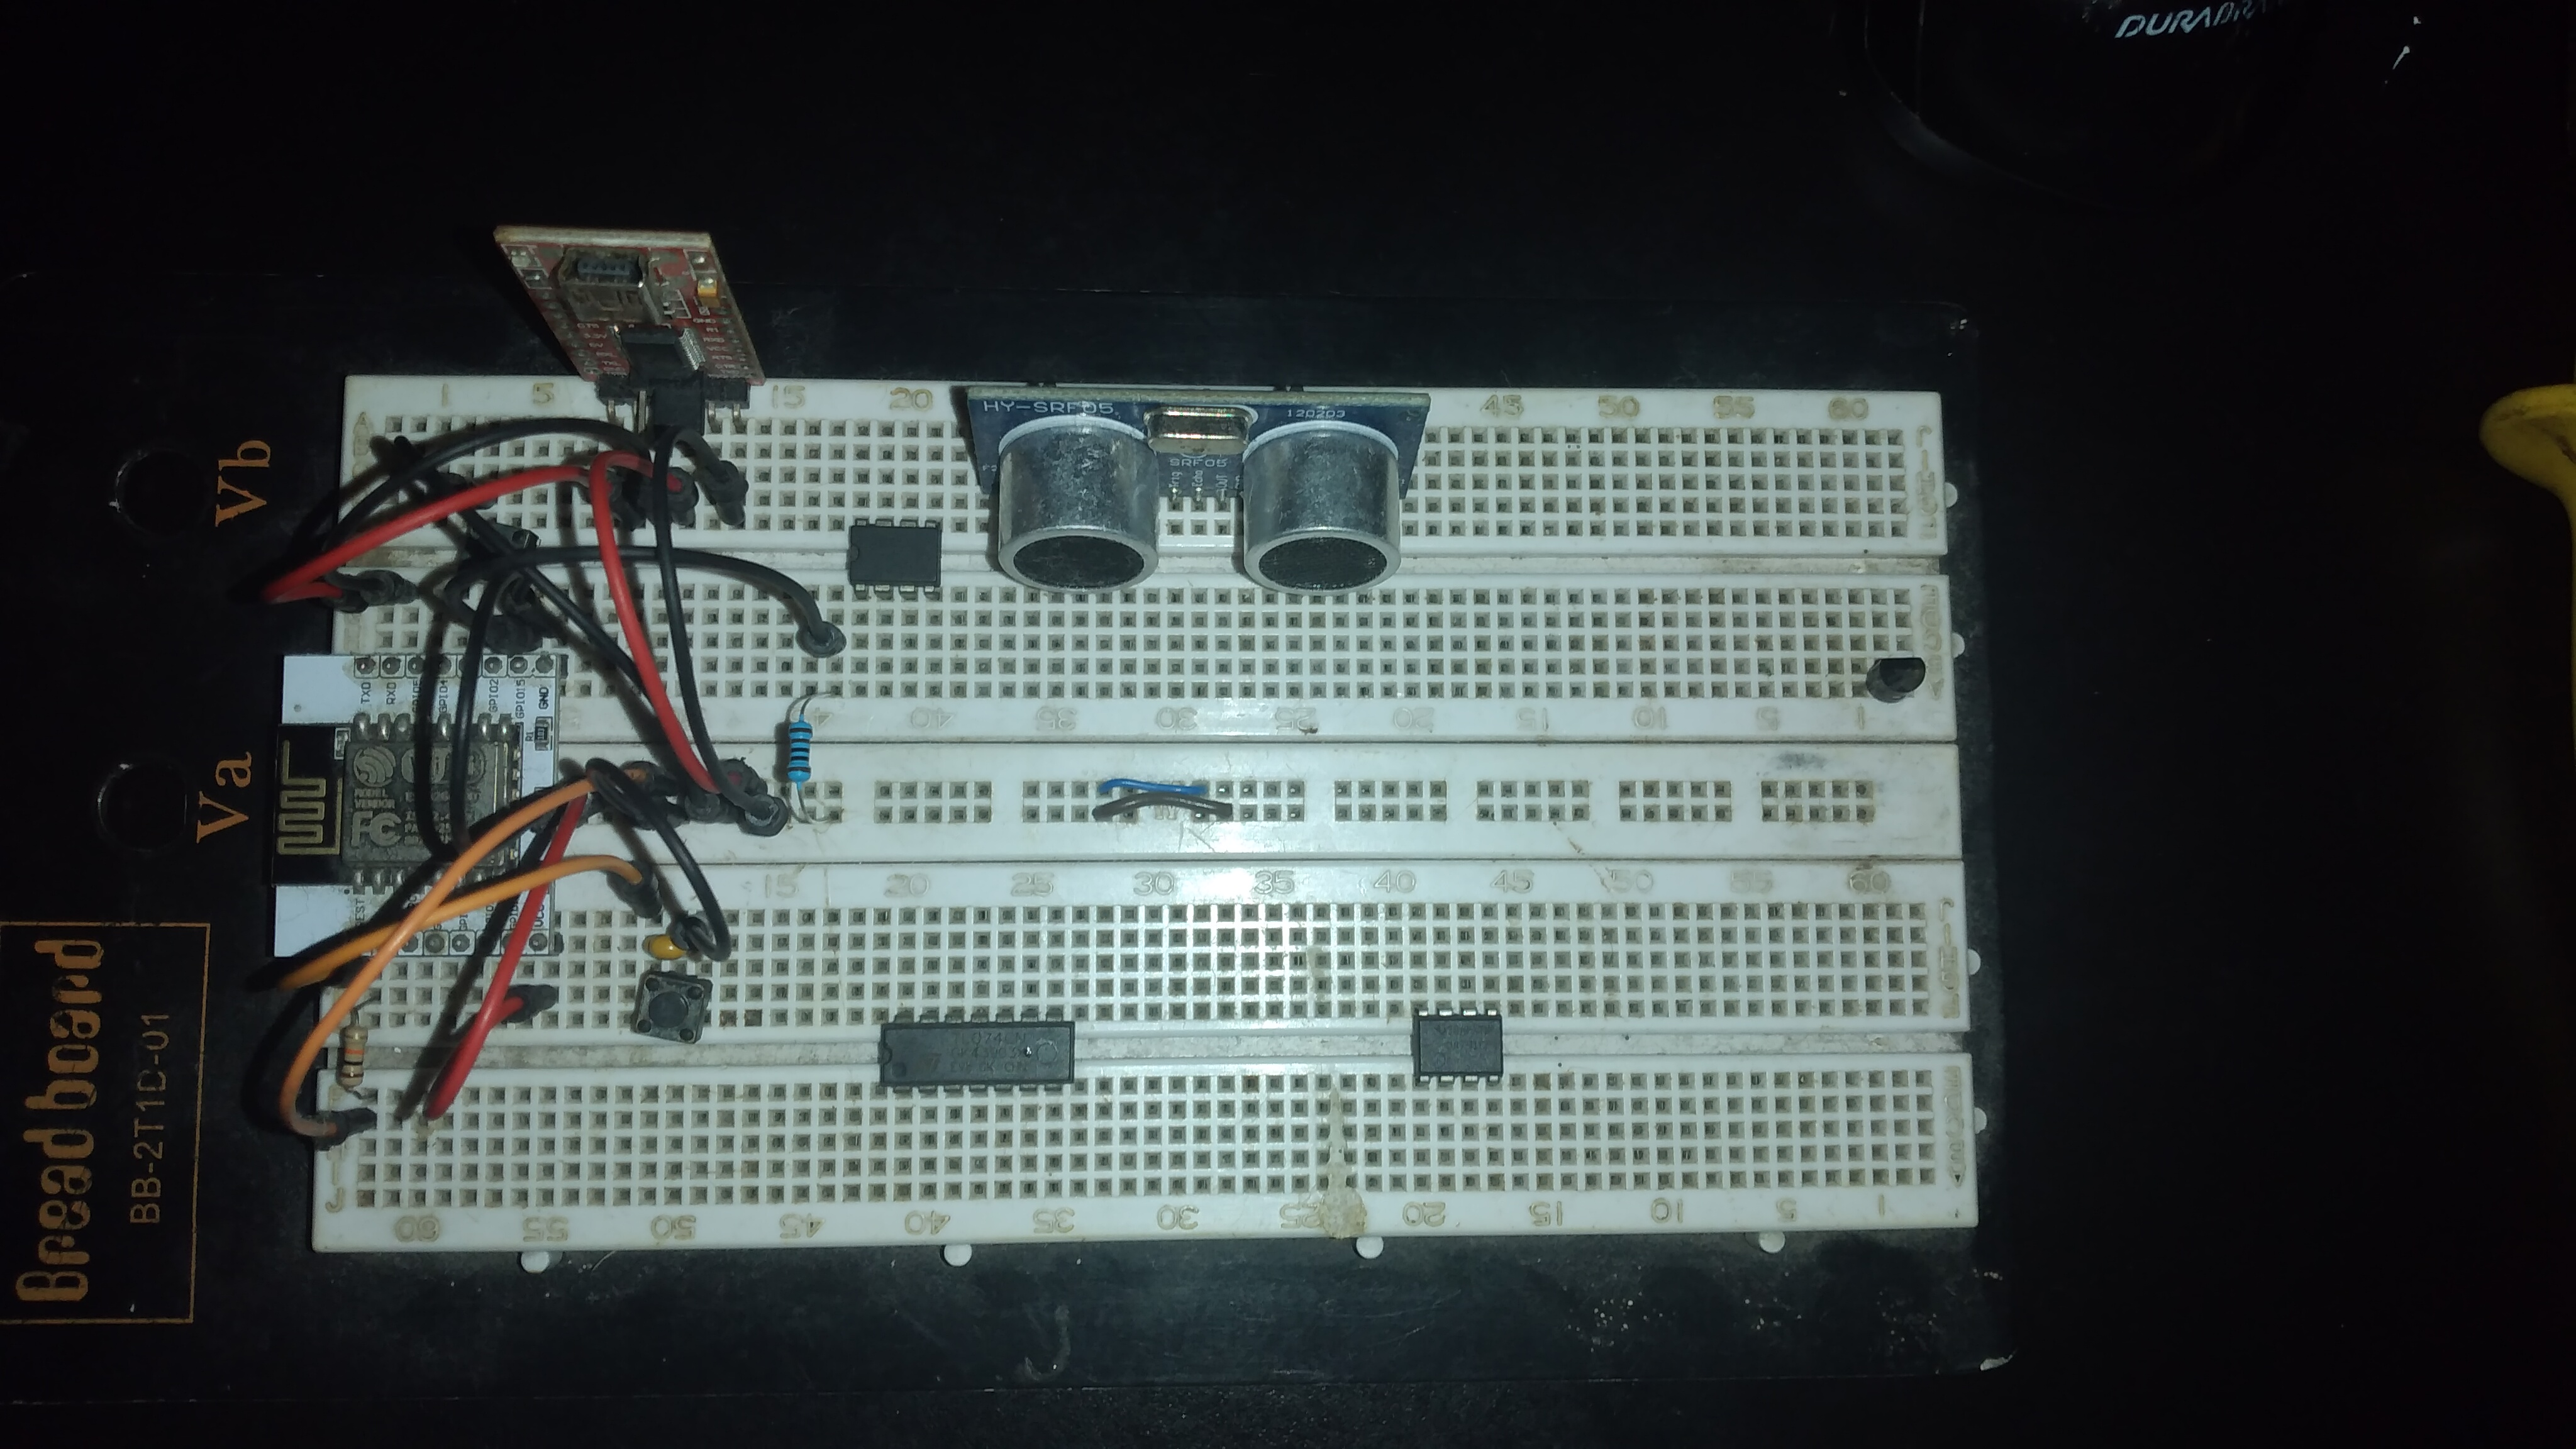
\includegraphics[scale=0.05]{images/20231001_152253.jpg}
    \caption{ESP8266 para envío de datos al servidor}
\end{figure}

\begin{figure}[H]
    \centering
    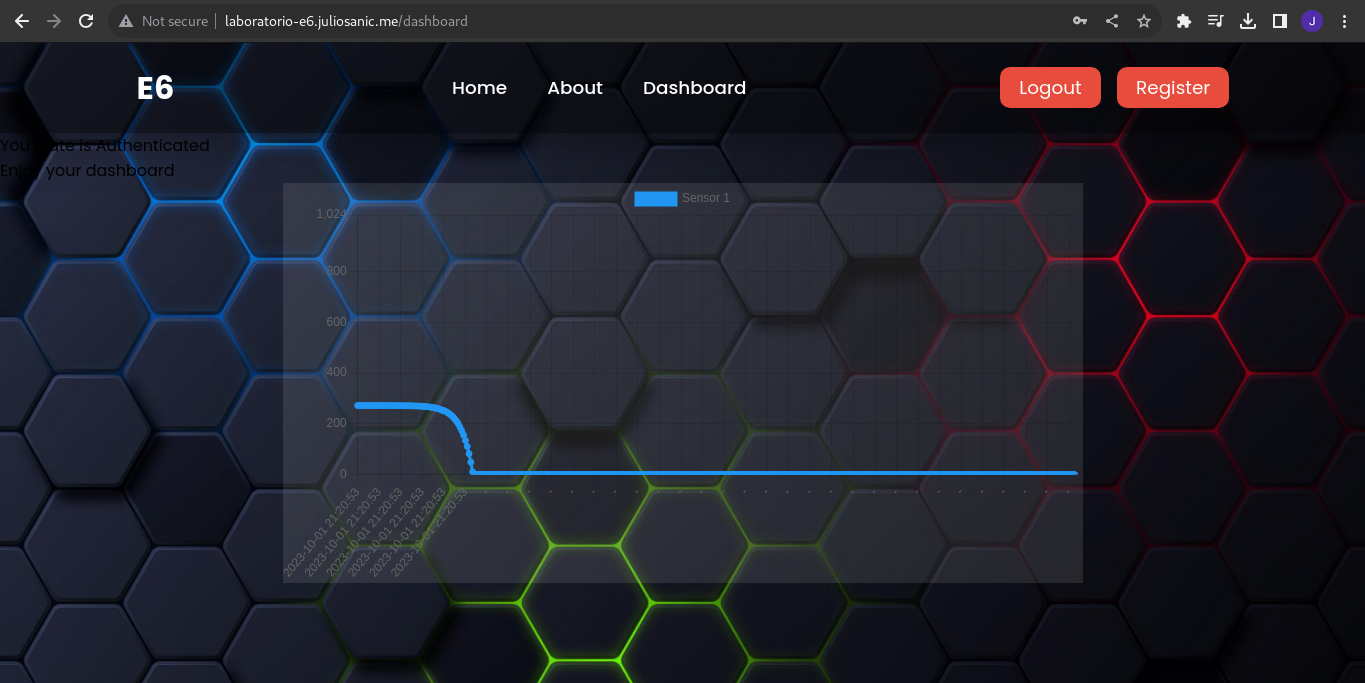
\includegraphics[scale=0.15]{images/dashboard.png}
    \caption{Página en ReactJS para la visualización de datos}
\end{figure}

\lstset{
  basicstyle=\ttfamily,
  keywordstyle=\color{blue}, % Use the defined color for keywords
  commentstyle=\itshape\color{green!60!black},
  stringstyle=\color{orange},
  numbers=left,
  numberstyle=\tiny,
  numbersep=5pt,
  showstringspaces=false,
  breaklines=true,
  frame=single,
  frameround=tttt,
  xleftmargin=15pt,
  xrightmargin=15pt,
  columns=fullflexible,
  linewidth=0.9\linewidth, % Adjust the width as needed
  keepspaces=true,
  caption=Servidor websocket en node.js, % Add your caption
  captionpos=b % Position of the caption (b for below)
}
\lstinputlisting{code/backend/index.js}
\lstset{
  basicstyle=\ttfamily,
  keywordstyle=\color{blue}, % Use the defined color for keywords
  commentstyle=\itshape\color{green!60!black},
  stringstyle=\color{orange},
  numbers=left,
  numberstyle=\tiny,
  numbersep=5pt,
  showstringspaces=false,
  breaklines=true,
  frame=single,
  frameround=tttt,
  xleftmargin=15pt,
  xrightmargin=15pt,
  columns=fullflexible,
  linewidth=0.9\linewidth, % Adjust the width as needed
  keepspaces=true,
  caption=Almacenamiento de datos esp8266 a servidor, % Add your caption
  captionpos=b % Position of the caption (b for below)
}
\lstinputlisting{code/backend/mqtt_program.js}
\lstset{
  basicstyle=\ttfamily,
  keywordstyle=\color{blue}, % Use the defined color for keywords
  commentstyle=\itshape\color{green!60!black},
  stringstyle=\color{orange},
  numbers=left,
  numberstyle=\tiny,
  numbersep=5pt,
  showstringspaces=false,
  breaklines=true,
  frame=single,
  frameround=tttt,
  xleftmargin=15pt,
  xrightmargin=15pt,
  columns=fullflexible,
  linewidth=0.9\linewidth, % Adjust the width as needed
  keepspaces=true,
  caption=Programa multihilo para ejecutar servidor websocket y alcamenamiento de datos, % Add your caption
  captionpos=b % Position of the caption (b for below)
}
\lstinputlisting{code/backend/main.js}

\lstset{
  language=C++,
  basicstyle=\ttfamily,
  keywordstyle=\color{blue}, % Use the defined color for keywords
  commentstyle=\itshape\color{green!60!black},
  stringstyle=\color{orange},
  numbers=left,
  numberstyle=\tiny,
  numbersep=5pt,
  showstringspaces=false,
  breaklines=true,
  frame=single,
  frameround=tttt,
  xleftmargin=15pt,
  xrightmargin=15pt,
  columns=fullflexible,
  linewidth=0.9\linewidth, % Adjust the width as needed
  keepspaces=true,
  caption=Configuración de red esp8266, % Add your caption
  captionpos=b % Position of the caption (b for below)
}
\lstinputlisting{code/esp8266/config.h}

\lstset{
  language=C++,
  basicstyle=\ttfamily,
  keywordstyle=\color{blue}, % Use the defined color for keywords
  commentstyle=\itshape\color{green!60!black},
  stringstyle=\color{orange},
  numbers=left,
  numberstyle=\tiny,
  numbersep=5pt,
  showstringspaces=false,
  breaklines=true,
  frame=single,
  frameround=tttt,
  xleftmargin=15pt,
  xrightmargin=15pt,
  columns=fullflexible,
  linewidth=0.9\linewidth, % Adjust the width as needed
  keepspaces=true,
  caption=Configuración esp8266 en modo station, % Add your caption
  captionpos=b % Position of the caption (b for below)
}
\lstinputlisting{code/esp8266/ESP8266_Utils_MQTT.hpp}

\lstset{
  language=C++,
  basicstyle=\ttfamily,
  keywordstyle=\color{blue}, % Use the defined color for keywords
  commentstyle=\itshape\color{green!60!black},
  stringstyle=\color{orange},
  numbers=left,
  numberstyle=\tiny,
  numbersep=5pt,
  showstringspaces=false,
  breaklines=true,
  frame=single,
  frameround=tttt,
  xleftmargin=15pt,
  xrightmargin=15pt,
  columns=fullflexible,
  linewidth=0.9\linewidth, % Adjust the width as needed
  keepspaces=true,
  caption=Configuración mqtt esp8266, % Add your caption
  captionpos=b % Position of the caption (b for below)
}
\lstinputlisting{code/esp8266/ESP8266_Utils_MQTT.hpp}

\lstset{
  language=C++,
  basicstyle=\ttfamily,
  keywordstyle=\color{blue}, % Use the defined color for keywords
  commentstyle=\itshape\color{green!60!black},
  stringstyle=\color{orange},
  numbers=left,
  numberstyle=\tiny,
  numbersep=5pt,
  showstringspaces=false,
  breaklines=true,
  frame=single,
  frameround=tttt,
  xleftmargin=15pt,
  xrightmargin=15pt,
  columns=fullflexible,
  linewidth=0.9\linewidth, % Adjust the width as needed
  keepspaces=true,
  caption=Configuración principal MQTT, % Add your caption
  captionpos=b % Position of the caption (b for below)
}
\lstinputlisting{code/esp8266/MQTT.hpp}

\lstset{
  language=C++,
  basicstyle=\ttfamily,
  keywordstyle=\color{blue}, % Use the defined color for keywords
  commentstyle=\itshape\color{green!60!black},
  stringstyle=\color{orange},
  numbers=left,
  numberstyle=\tiny,
  numbersep=5pt,
  showstringspaces=false,
  breaklines=true,
  frame=single,
  frameround=tttt,
  xleftmargin=15pt,
  xrightmargin=15pt,
  columns=fullflexible,
  linewidth=0.9\linewidth, % Adjust the width as needed
  keepspaces=true,
  caption=Configuración de red esp8266, % Add your caption
  captionpos=b % Position of the caption (b for below)
}
\lstinputlisting{code/esp8266/config.h}

\lstset{
  basicstyle=\ttfamily,
  keywordstyle=\color{blue}, % Use the defined color for keywords
  commentstyle=\itshape\color{green!60!black},
  stringstyle=\color{orange},
  numbers=left,
  numberstyle=\tiny,
  numbersep=5pt,
  showstringspaces=false,
  breaklines=true,
  frame=single,
  frameround=tttt,
  xleftmargin=15pt,
  xrightmargin=15pt,
  columns=fullflexible,
  linewidth=0.9\linewidth, % Adjust the width as needed
  keepspaces=true,
  caption=Componente React principal para cliente websocket, % Add your caption
  captionpos=b % Position of the caption (b for below)
}
\lstinputlisting{code/frontend/ChartJsExample.jsx}
\subsection{Bocina}


\begin{figure}[H]
    \centering
    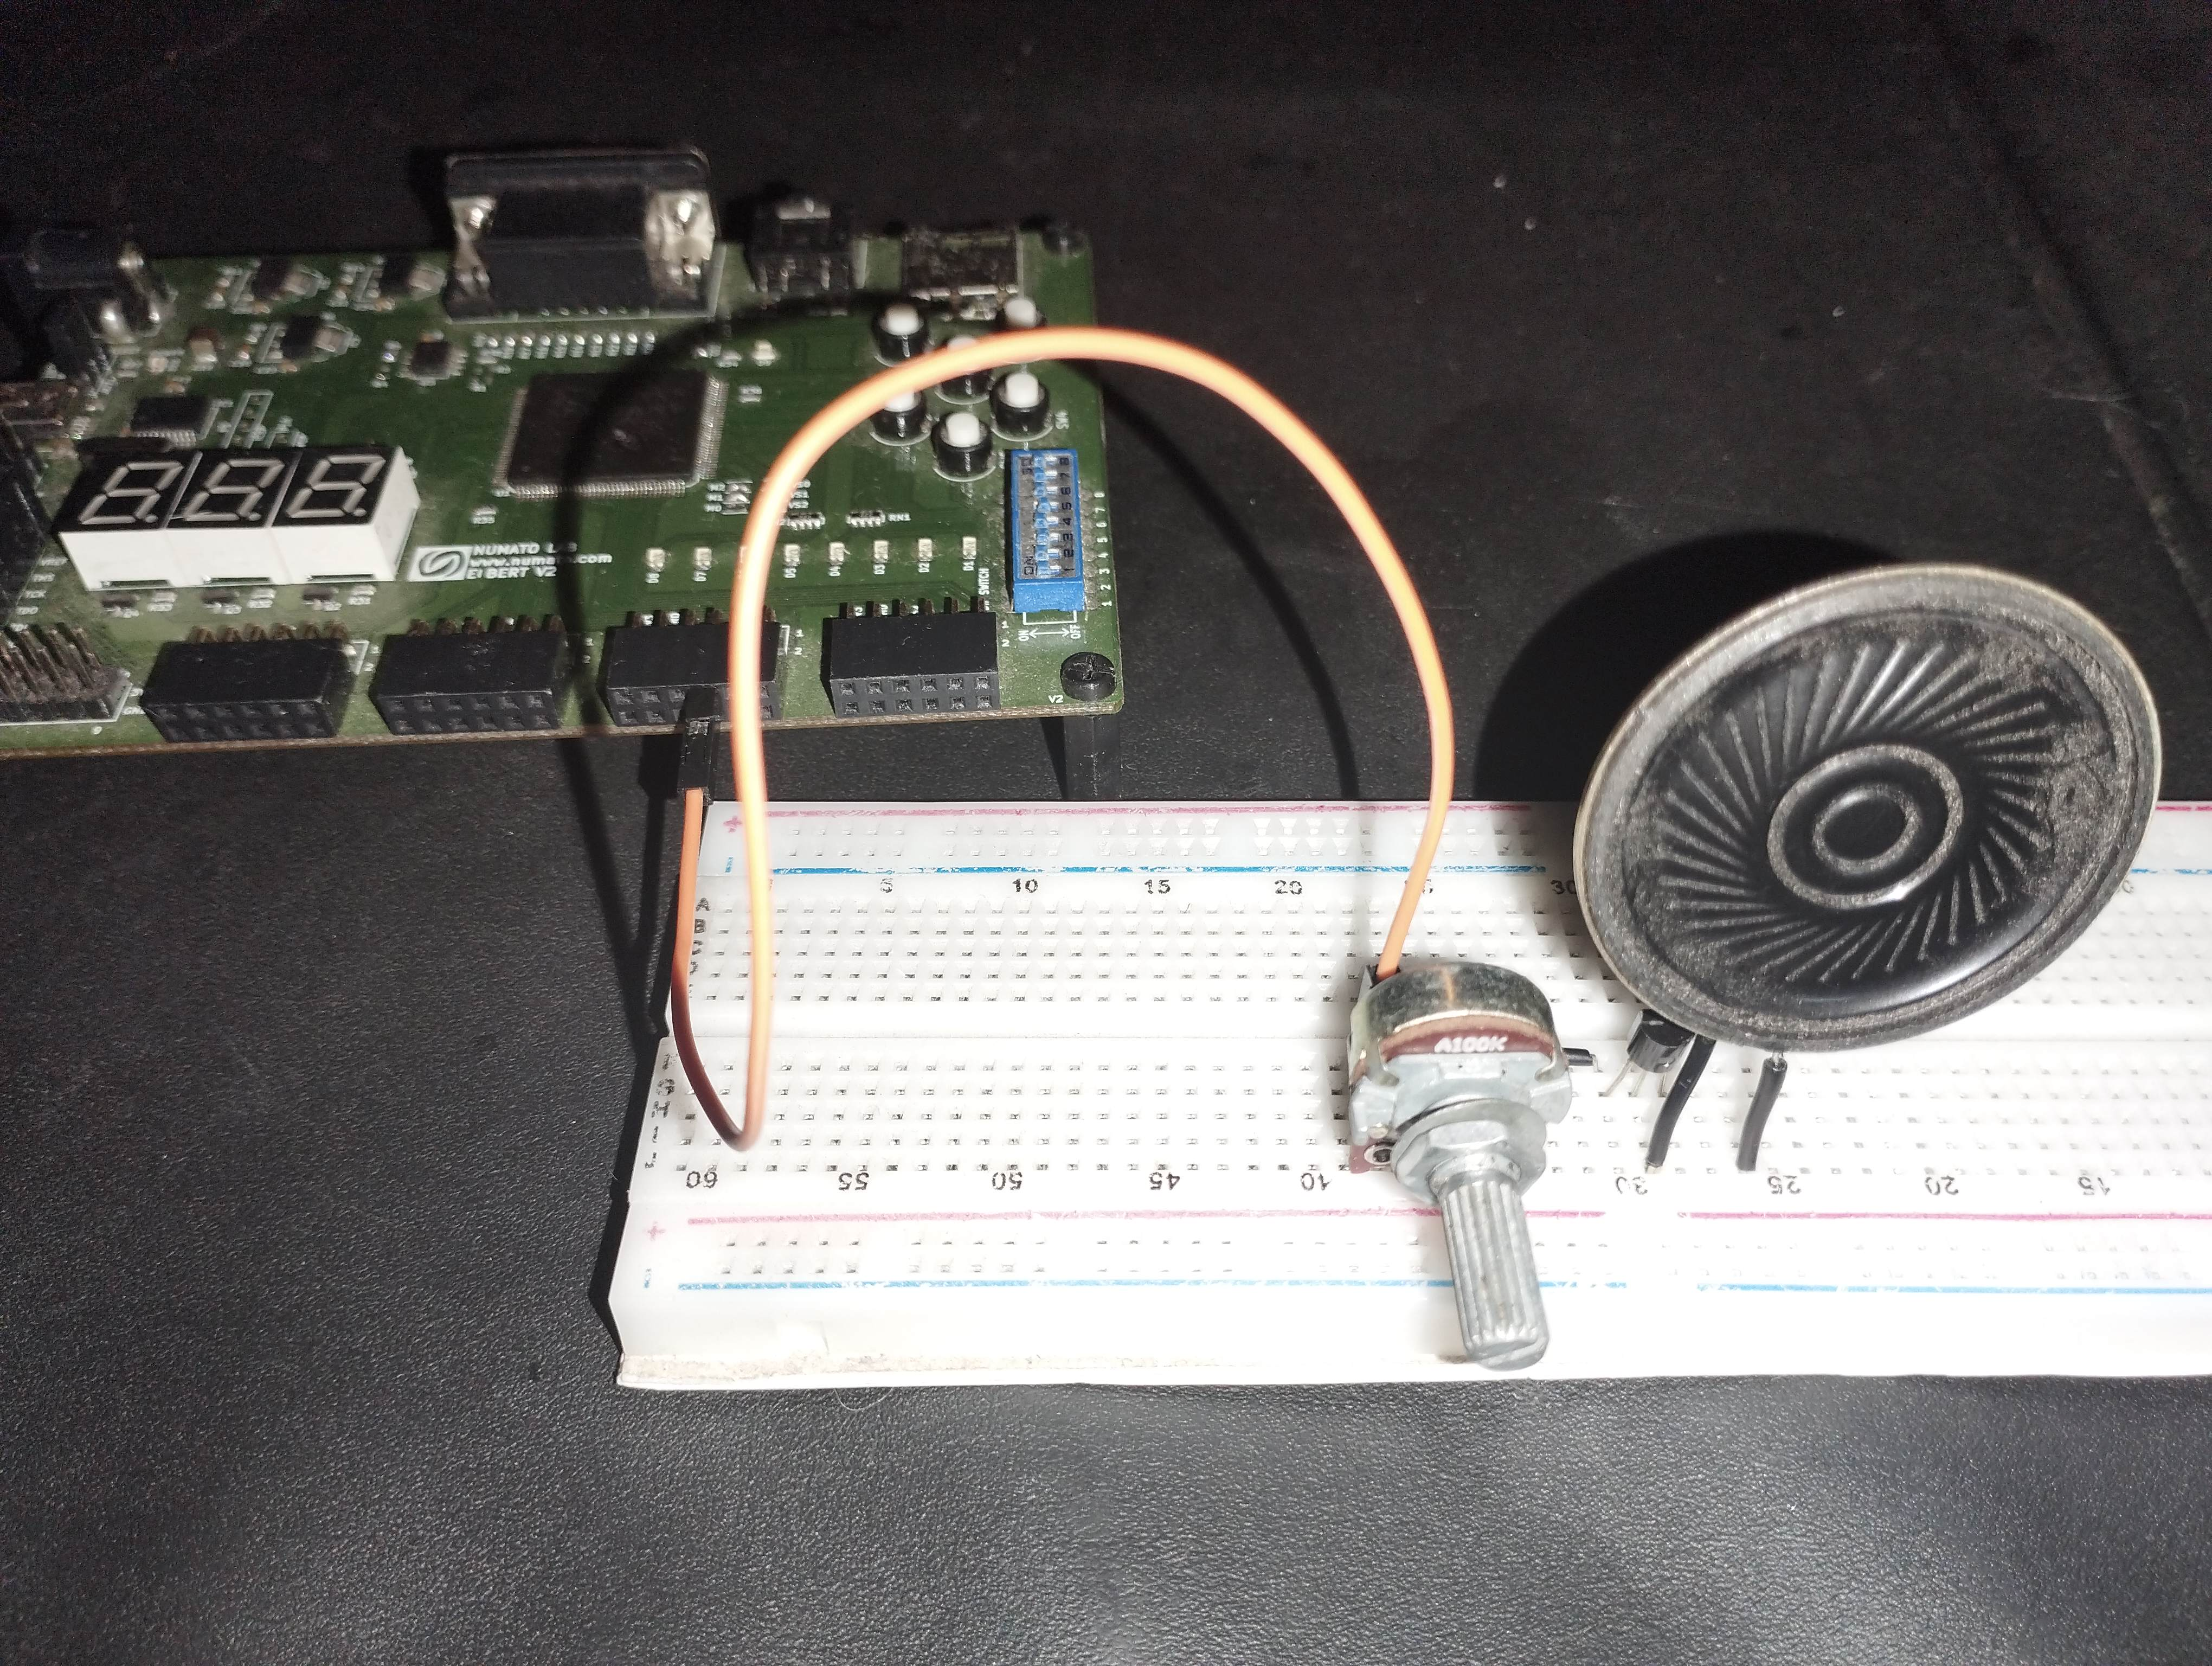
\includegraphics[scale=0.04]{images/IMG_20231001_163603.jpg}
    \caption{Conexiones posibles para bocina}
\end{figure}

\begin{figure}[H]
    \centering
    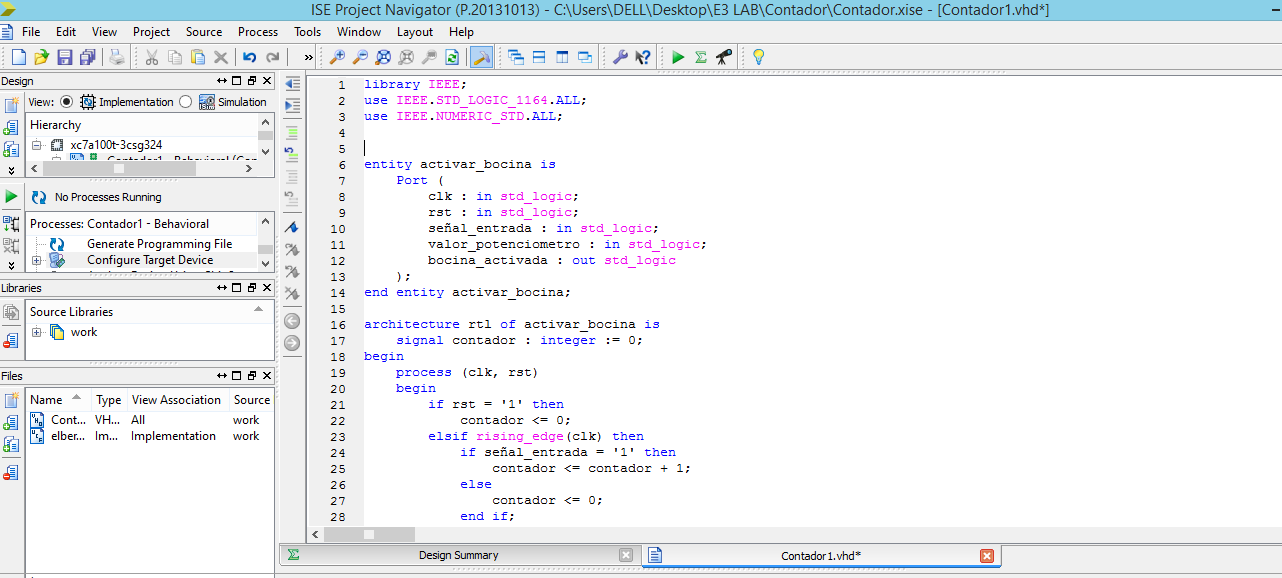
\includegraphics[scale=0.2]{images/2.png}
    \caption{Código para activacion de bocina}
\end{figure}

\begin{figure}[H]
    \centering
    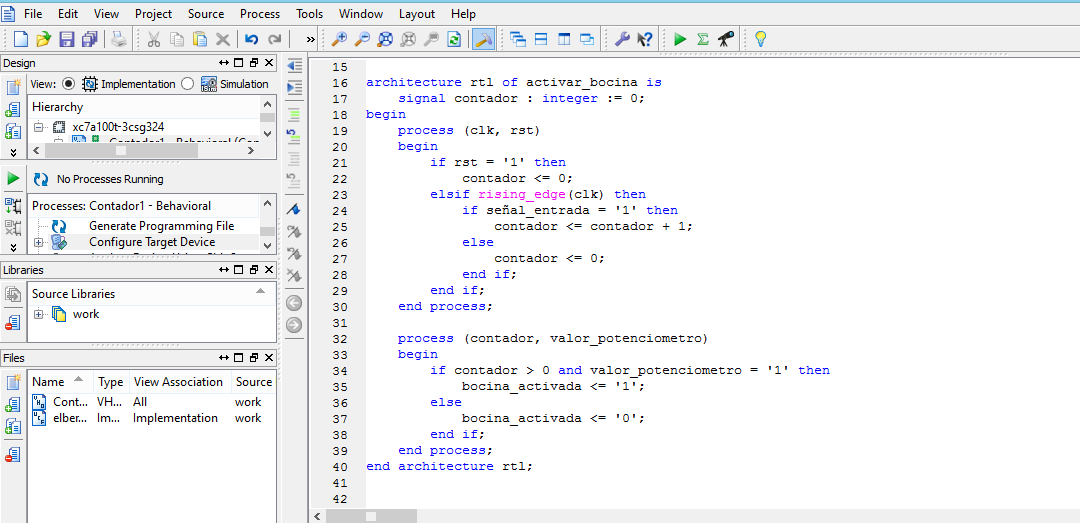
\includegraphics[scale=0.2]{images/3.png}
    \caption{Código para activacion de bocina}
\end{figure}

\section{Conclusiones}
\begin{itemize}
    \item A través del análisis de la teoría aplicada en el sistema de la maqueta virtual, se comprende que es necesario la adaptación de sensores ultrasonicos HC-SR04, para la incorporación del GPS a usar
    
    \item La comprensión de la estructura física del uso de sistemas de maquetación permite comprender el uso de los dispositivos actuantes en la interfaz conectada hacia la placa, por lo permite detallar y optimizar la codificación utilizada. 
    
    \item Las demostraciones usadas en la evlacuación de los elementos electronicos utilizados permite comprender los usos y aplicaciones del lenguaje ensamblador en sistemas controlas.

\end{itemize}

\begin{thebibliography}{99}
%Las fuentes de consulta se citan en forma organizada y homogénea, tanto de los libros, de los artículos y, en general, de las obras consultadas, que fueron indispensables indicar o referir en el contenido del trabajo.
\bibitem{} Boylestad.R.L. 2011. \textit{Introducción al Análisis de Circuitos}. 12mo Ed. PEARSON. México.

\bibitem{} Boylestad.R.L. 2010. \textit{Electrónica: Teoría de Circuitos y Dispositivos Electrónicos}. 10mo Ed. PEARSON. México.

\bibitem{} González Ermakov, M. (2019). Modulación por ancho de pulso de alta resolución en FPGA (Bachelor's thesis). 

\bibitem{} Flanagan, D. 2011. \textit{JavaScript: The Definitive Guide}. 6ta Ed. O'Reilly Media. 

\bibitem{} Van Rossum, G. 2010. \textit{Python Programming for the Absolute Beginner}. 3ra Ed. Course Technology.

\bibitem{} Rauch, R., \& Kirk, T. 2018. \textit{Node.js Design Patterns}. 3ra Ed. Packt Publishing.

\end{thebibliography}

\end{document}